\documentclass{article}
\usepackage{graphicx}
\usepackage[utf8]{inputenc}
\usepackage[fleqn]{amsmath}
\usepackage{titling}
\usepackage{graphicx,wrapfig,lipsum}
\usepackage{amssymb}
\usepackage{listings}
\usepackage[font=small,labelsep=none]{caption}
\usepackage{hyperref}
\usepackage{caption}

\setlength{\droptitle}{-10em}
\setlength\parindent{0pt}

\title{Project 2}\vspace{-3ex}
\author{Benedicte Allum Pedersen, Emil Heland Broll\\ Fredrik Oftedal Forr}
\date{\vspace{-5ex}}

\begin{document}
\maketitle

\section{Abstract}
	We have developed a program using the Jacobi method for solving eigenvalue problems, from the equations of a buckling beam to Schroedinger's equation for two electrons in a three-dimensional harmonic oscillator well. We discover that the Jacobi method and Armadillo's eigensystem-solver gives the exact same eigenvalues, but the runtime for Jacobi's method is a lot higher.

\section{Introduction}
	In this project we will solve eigenpair-problems using numerical calculations. We will also implement unit testing in our code to avoid mathematical and programming errors. We begin by explaining the theoretical models and algorithms we use to compute the eigenvalues,
	along with technicalities related to the programming of these models. We will then present and discuss our results, before finally reaching a conclusion regarding the methods we use
	in terms of efficiency and precision.

\section{Methods}
	\subsection{Mathematics}
		We will start off by proving that orthogonal or unitary transformations preserves
		the orthogonality of the vectors.

		Starting with an orthogonal basis of vectors, $\textbf{v}_i$, we know that:

		\begin{flalign*}
		\begin{aligned}
			\textbf{v}_i = \begin{bmatrix}
			v_{i1} \\
			\vdots \\
			v_{in}
			\end{bmatrix},
		\end{aligned}
		\qquad
		\begin{aligned}
			\textbf{v}_j^T \textbf{v}_i = \delta_{ij}
		\end{aligned}
		\end{flalign*}

		An orthogonal transformation gives us the following:
		\begin{flalign*}
		&\textbf{w}_i=U\textbf{v}_i, \text{where } U^TU=UU^T=\textbf{I}
		\end{flalign*}

		We want to prove that orthogonality is preserved:
		\begin{flalign*}
		\textbf{w}_i^T \textbf{w}_j = (U\textbf{v}_i)^T (U\textbf{v}_j) = \textbf{v}_i^T U^T U \textbf{v}_j = \textbf{v}_i^T \textbf{v}_j
		\end{flalign*}

		Now that we have proved that orthogonal transformations preserve orthogonality,
		we can move on to performing our Jacobi iterations.
		To do so, we use an orthogonal transformation matrix, S:
		\begin{flalign*}
			S = \begin{bmatrix}
				1 & 0 & \cdots \\
				0 & 1 &  0 \\
				\vdots & 0 & \ddots \\
				& & & \cos{\theta} & 0 & \cdots & \sin{\theta} \\
				& & & 0 & 1 & \cdots & 0 \\
				& & & \vdots & \vdots & \ddots & \vdots \\
				& & & -\sin{\theta} & 0 & \cdots & \cos{\theta}
			\end{bmatrix}, \qquad S^T=S^{-1}
		\end{flalign*}

		We simplify by assigning:
		\begin{flalign*}
			c = \cos{\theta}, s = \sin{\theta}, t = \tan{\theta} = \frac{s}{c}
		\end{flalign*}

		For our positive definite matrix ${A}$, we perform the transformation
		\\${S^TA S = B}$, giving us the general expression:
		\begin{flalign*}
		&	b_{ii} = a_{ii}, i \neq k, i \neq l \\
		&	b_{ik} = a_{ik}c - a_{il} s, i \neq k, i\neq l \\
		&	b_{il} = a_{il} c + a_{ik} s, i \neq k, i\neq l \\
		&	b_{kk} = a_{kk} c^2 - 2a_{kl}cs + a_{ll} s^2 \\
		&	b_{ll} = a_{ll} c^2 - 2a_{kl}cs + a_{kk} s^2 \\
		&	b_{kl} = (a_{kk}-a_{ll})cs + a_{kl}(c^2-s^2)
		\end{flalign*}

		By choosing the largest non-diagonal element in the original matrix $A$,
		we can fix $\theta$ by choosing to set the largest non-diagonal element to zero.
		From this, we can deduce the required values of $c$ and $s$:
		\begin{flalign*}
			c = \frac{1}{\sqrt(1+t^2)}, \qquad s = tc \\
			t = -\tau \pm \sqrt{1+\tau^2}, \qquad \tau = \frac{a_{ll}-a_{kk}}{2a_{kl}}
		\end{flalign*}

		This will result in a new matrix, B. We can then find the largest non-diagonal element
		of the new matrix and repeat the algorithm until this value is less than a given tolerance.
		\begin{flalign*}
			B_2 = S_2^T B S_2
		\end{flalign*}

		When this is achieved, we will have a diagonal matrix, where all non-diagonal matrix elements
		are approaching 0.
		\begin{flalign*}
			D = S_n^T S_{n-1}^T \cdots S_1^T A S_1 \cdots S_{n-1} S_n
		\end{flalign*}

		Since we have only performed orthogonal transformations,
		the eigenvaluesfor $D$ and $A$ will be the same.
		Since diagonal matrices have their eigenvalues on the diagonal, we can easily read off the eigenvalues.\\

		\subsubsection{Quantum dots in three dimensions, one electron}
			We will now consider a physical application of our algorithm by adapting it
			in order to solve the three dimensional Schrödinger Equation.
			The general radial form of this equation is:
			\begin{flalign*}
				-\frac{\hbar^2}{2m} \left(\frac{1}{r^2} \frac{d}{dr}r^2 \frac{d}{dr}-\frac{l(l+1)}{r^2}\right) R(r) + V(r) R(r) = E R(r)
			\end{flalign*}

			We can now do a series of subtitutions and insert some boundary conditions. We assume $l=0$.
			\begin{flalign*}
			&	R(r) = \frac{1}{r} u(r), \qquad u(0) = u(\infty) = 0\\
			&	\rho = \frac{1}{\alpha} r\\
			&	V(\rho) = \frac{1}{2} k \alpha^2 \rho^2\\
			&	\frac{mk}{\hbar^2} \alpha^4 = 1 \Rightarrow \alpha = \left( \frac{\hbar^2}{mk} \right)^{1/4}\\
			&	\lambda = \frac{2m\alpha^2}{\hbar^2} E
			\end{flalign*}

			We can then rewrite the Schröedinger Equation like this:
			\begin{flalign*}
				- \frac{d^2}{d\rho^2} u(\rho) + \rho^2 u(\rho) = \lambda u(\rho)
			\end{flalign*}

			We can now discretise this equation by defining the step length $h$ and $\rho_{min}=\rho_0$.
			We also need to approximate $\infty$, as the computer cannot represent infinity: $p_{max} = \rho_N$.
			\begin{flalign*}
				h = \frac{\rho_N - \rho_0}{N}\\
				\rho_i = \rho_0 + ih, \qquad i = 1, \hdots, N
			\end{flalign*}

			The Schröedinger equation now becomes:
			\begin{flalign*}
				- \frac{u_{i+1} - 2u_i + u_{i-1}}{h^2} + V_i u_i = \lambda u_i
			\end{flalign*}

			Where $u_i = u(\rho_i)$ and $u_{i\pm 1} = u(\rho_i) \pm h$ and $V_i = \rho_i^2$.
			We can then see that the Schröedinger equation can be simplified even more:
			\begin{flalign*}
				d_i u_i + e_i u_{i-1} + e_i u_{i+1} = \lambda u_i\\
				d_i = \frac{2}{h^2} + V_i\\
				e_i = - \frac{1}{h^2} = e
			\end{flalign*}

			Where $d_i$ are the diagonal elements of our tridiagonal matrix, and $e_i$ are
			the non-diagonal elements, which are all equal.
			This lets us rewrite the Schröedinger equation as a linear problem:

			\begin{equation*}
				\begin{bmatrix}
					d_1 & e & 0   & 0    & \dots  &0     & 0 \\
					e & d_2 & e & 0    & \dots  &0     &0 \\
					0   & e & d_3 & e  &0       &\dots & 0\\
					\dots  & \dots & \dots & \dots  &\dots      &\dots & \dots\\
					0   & \dots & \dots & \dots  &\dots  e     &d_{N-2} & e\\
					0   & \dots & \dots & \dots  &\dots       &e & d_{N-1}
				\end{bmatrix}
				\begin{bmatrix}
					u_{1} \\
					u_{2} \\
					\dots\\ \dots\\ \dots\\
					u_{N-1}
				\end{bmatrix}
				= \lambda \begin{bmatrix}
					u_{1} \\
					u_{2} \\
					\dots\\ \dots\\ \dots\\
					u_{N-1}
				\end{bmatrix}
				\label{eq:sematrix}
			\end{equation*}

			We can now see that we can use our algorithm to solve our radial Schröedinger equation.
			We can then run our algorithms with different number of integration points,
			$N$, and the approximation to $\infty$, $\rho_{max}$.\\
			The resulting $\lambda$ values are unitless numbers,
			which can be tranformed back into energies by using the value $\alpha$.

		\subsubsection{Quantum dots in three dimensions, two electrons}
			If we now consider a system with two electrons,
			the electron repulsion between them will come into play in the Schröedinger equation.
			By doing a lot of the equivalent substitutions and rewriting the equation,
			we get to a point where we end up with a linear problem,
			with a tridiagonal matrix with diagonal elements:
			\begin{equation*}
				d_i = \frac{2}{h^2} + \omega_r^2 \rho^2 + 1/\rho
			\end{equation*}

			Here, $\omega_r$ represents the strength of the oscillator potential.
			We will study the cases $\omega_r = 0.01, 0.5, 1, 5$, for the ground state ($l = 0$),
			and compare these to known analytical solutions of the problem.

	\subsection{Programming}
		To avoid errors in our code, we implement unit tests at the following points:
		\begin{itemize}
			\item Testing the max\_offdiag-function to confirm it locates the largest non-diagonal element
			\item Testing that the eigenvalues our eigensolver finds are within a given tolerance of the analytical values
		\end{itemize}
		The link to our GitHub repository where you can find our codes are found in the bibliography.

\section{Results, discussion}
	For our eigenproblem-solver, we tested and found a reasonable tolerance,
	$10^{-8}$, so that the algorithm converges without reaching the maximum number of iterations,
	$n^3$. We test this using a tridiagonal matrix:
	\begin{flalign*}
		A =   \begin{bmatrix}
			2 & -1 & 0 &\dots & 0 & 0\\
			-1 & 2 & -1 & \dots & 0 & 0\\
			0 & -1 & 2 & \dots & 0 & 0 \\
			\vdots & \vdots & \vdots & \ddots & \vdots & \vdots \\
			0 & 0 & 0 &\dots& 2 & -1\\
			0 & 0 & 0 &\dots& -1 & 2
		\end{bmatrix}
	\end{flalign*}

	Table 1 shows the number of similarity transformations were needed
	to reach a point where all non-diagonal matrix elements approach 0, for the matrix $A$ with different dimensionalities.

	\begin{table}[h!]
		\caption{: Dimensionality and number of similarity transformations required to reach the tolerance.}
		\begin{tabular}{c c c}
			Dimensionality & \# of transformations\\
			\hline
			4 & 6 \\
			10 & 141 \\
			20 & 551 \\
			50 & 3529
		\end{tabular}
	\end{table}

	By using polynomial regression, see figure 1, we can see that it looks like
	$i(n) = 1.49n^2 - 1.63n - 4.23$, where $i$ is number of iterations
	and $n$ is dimensinality of the matix.\\

	\begin{figure}[hbt]
	\begin{center}
	    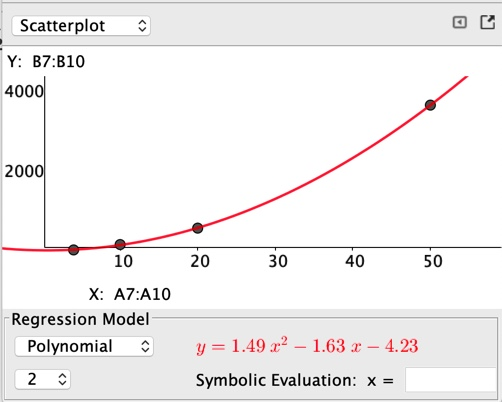
\includegraphics[width=200px]{bilde.jpg}
	    \caption{: Polynomial regression to obtain the equation for $i$ as a function of n when $y=i$ and $x=n$}
	    \label{fig:plot1b}
	\end{center}
	\end{figure}

	Table 2 shows a comparison of eigenvalues found with Armadillo's eigensystem-solver
	and our Jacobi rotating solver on our tridiagonal matrix A.
	\begin{table}[h!]
		\caption{: Eigenvalues using the Jacobi method and Armadillo for $n=5$.}
		\begin{tabular}{c c c}
			$\lambda_{\text{Jacobi}}$ & $\lambda_{\text{Armadillo}}$ & Analytical \\
			\hline
			0.2679 & 0.2679 & 0.26795 \\
			1.0000 & 1.0000 & 1 \\
			2.0000 & 2.0000 & 2 \\
			3.0000 & 3.0000 & 3 \\
			3.7321 & 3.7321 & 3.73205 \\
		\end{tabular}
	\end{table}

	Table 3 shows a comparison of runtimes of the Armadillo eigensystem-solver and our diagonalisation, for a 50x50-matrix.

	\begin{table}[h!]
		\caption{: Runtimes using the Jacobi method and Armadillo, for $n=1000$.}
		\begin{tabular}{c c}
			Jacobi runtime & Armadillo runtime\\
			\hline
			5.6104s (14026 iterations) & 0.00287s
		\end{tabular}
	\end{table}

	\subsection{Quantum dots in three dimensions, one electron}
		Table 4 shows the reslults of finding the eigenvalues with the Armadillo solver with the modified diagonal matrix elements
		of the Schröedinger equation, while varying the number of integration points, $N$. \\
		Table 5 shows the reslult while varying the approximation of $\rho_{max} = \infty$. \\
		The analytical eigenvalues are:
		\begin{equation*}
			\lambda = 3,7,11,15,\hdots
		\end{equation*}


		\begin{table}[h!]
			\caption{: Numerical eigenvalues, varying N ($\rho_{max} = 10$)}
			\begin{tabular}{c c c}
				$\lambda_{N=10000}$ & $\lambda_{N=1200}$ & $\lambda_{N=900}$ \\
				\hline
				3.0000 & 2.9998 & 2.9996  \\
				6.9999 & 6.9990 & 6.9983  \\
				11.0000 & 10.9976 & 10.9958  \\
				14.9999 & 14.9956 & 14.9956  \\
			\end{tabular}
		\end{table}
		\begin{table}[h!]
			\caption{: Numerical eigenvalues, varying $\rho_{max}$ ($N = 1200$).}
			\begin{tabular}{c c c}
				$\lambda_{\rho_{max} = 5}$ & $\lambda_{\rho_{max} = 10}$ & $\lambda_{\rho_{max} = 50}$\\
				\hline
				2.9999 & 2.9999 & 2.9996 \\
				6.9999 & 6.9999 & 6.9983 \\
				11.0001 & 10.9997 & 10.9958 \\
				15.0060 & 14.9995 & 14.992 \\
			\end{tabular}
		\end{table}


	\subsection{Quantum dots in three dimensions, two electrons}
		Through trial and error, we determine the ideal $N = 1000$ and $\rho_{max} = 100$.
		Varying the strengths of $\omega_r$, we get the results in table 6.

		\begin{table}[h!]
			\caption{: Numerical eigenvalues, varying $\omega_{r}$)}
			\begin{tabular}{c c}
				$\omega_r$ & $E' = \lambda$ \\
				\hline
				0.01 & 0.3120 \\
				0.50 & 2.2301 \\
				1.00 & 4.0579 \\
			  	5.00 & 17.4485 \\
			\end{tabular}
		\end{table}


				\begin{table}[h!]
					\caption{: Numerical eigenvalues, varying $\omega_{r}$, and $\rho_{max} = 100$)}
					\begin{tabular}{c c c}
						$1/\omega_{r}$ & $\omega_r$ & $E' = \lambda$ \\
						\hline
						4 & 0.25 & 1.2500 \\
						20 & 0.05 & 0.3500 \\
						54.7386 & 0.018 & 0.1626 \\
						115.299 & 0.009 & 0.09799 \\
					\end{tabular}
				\end{table}

		\begin{table}[h!]
			\caption{: Analytical eigenvalues (\href{http://prola.aps.org/abstract/PRA/v48/i5/p3561_1}{M. Taut, Phys. Rev. A 48, 3561 (1993)}).}
			\begin{tabular}{c c c}
				$1/\omega_{r}$ & $\omega_r$ & $E' = \lambda$ \\
				\hline
				4 & 0.25 & 1.250\\
				20 & 0.05 & 0.350 \\
				54.7386 & 0.018 & 0.1644 \\
				115.299 & 0.009 & 0.0954 \\
			\end{tabular}
		\end{table}


\section{Conclusions, perspectives}
	We discovered that our eigenvalue solver gave the exact same values as
	the Armadillo eigensystem-solver, to a four decimal precision.\\
	Our algorithm was however a lot slower, approximately 2000 times slower for a $n=100$ matrix.
	This is probably to be expected, since the functionality is tailored for a dense,
	symmetrical matrix, while the Armadillo solver most likely has
	several optimization features which can utilize the simpler features of the Töeplitz matrix.\\
	To optimize our solver further, we can tailor it to a non-dense matrix, and one with identical non-diagonal elements, like we have througout this project.\\
	In order to effectively test and perform the calculations in the rest of the project, we have mainly used Armadillo's solver to get the values with the precision we wanted at a reasonable speed.\\

	We implemented two unit tests in the code, but we could also have included more to make sure the different parts of our code for this project was watertight. We could have performed the tests every time the code runs, just in case, but we felt that was overkill for this small project, so we made a separate test file we ran to check that these tests would pass. We could also have implemented a test for the 3D two-particle system, since we have analytical eigenvalues for this, and we could additionally have made a test that compares our algorithm's eigenvalues to those found by Armadillo, since we know they should be pretty accurate.\\\\

	For the 3D one-particle system, we varied the number of integration points/the dimensionality of the matrix while keeping the approximation of $\rho_{max}$ constant. We discovered that increasing the dimensionality gives better results, and $n=10000$ reproduces the analytical results within three decimal points. When varying $\rho_{max}$, we see that smaller values gives more precise results, with $\rho_{max} = 5, n=1200$ gives almost equally precise results as $\rho_{max} = 10, n=10000$. This is surprising to us, because one would expect a higher value of $\rho_{max}$ would give a better approximation of infinity, and therefore improve the results, but our findings show that the opposite happens. We struggeled to understand this.\\\\

	For the 3D two-particle system, by comparing the analytical and numerical eigenvalues, we discover that our model gives reasonable results for the different values of $\omega_r$ we test with. The larger values are more precise than the smaller ones, probably because of loss of numerical precision.\\\\

	In conclusion, our algorithm is not the most efficient, but it gives reasonable precision, and works fine. In general though, it would be better to use Armadillo's functions or other optimized existing algorithms, for quick and precise results.

\section{Bibliography}
	\href{http://prola.aps.org/abstract/PRA/v48/i5/p3561_1}{M. Taut, Phys. Rev. A 48, 3561 (1993)}.\\
	\href{https://github.com/emmernme/MENA-Compfys/tree/master/Project2}{Link to our GitHub repository}

\end{document}
